\documentclass[12pt, a4paper]{article}

\usepackage[utf8]{inputenc}
\usepackage{graphicx}
\usepackage{amsmath}
\usepackage{booktabs}
\usepackage{geometry}
\geometry{a4paper, top=1in, bottom=1in, left=1in, right=1in}
\usepackage{setspace}
\setstretch{1.5}
\usepackage[hidelinks]{hyperref}
\usepackage{cite}
\usepackage{float}

% Title Format
\usepackage{titlesec}
\titleformat{\section}{\Large\bfseries}{\thesection}{1em}{}
\titleformat{\subsection}{\large\bfseries}{\thesubsection}{1em}{}

\begin{document}

% --- Cover Page ---
\begin{titlepage}
    \centering
    \vspace*{2cm}
    
    \Huge
    \textbf{AI-Based Optimized Energy Utilization System Using Edge Computing Controllers}
    
    \vspace{1.5cm}
    
    \Large
    \textbf{EC8070 -- Research Project III}
    
    \vspace{2cm}
    
    \Large
    \textbf{E.M.I. Indrajith}\\
    \textbf{H.P.M. Hettiarachchi}
    
    \vspace{1.5cm}
    
    \textit{Supervisor:}\\
    \textbf{Dr. A. Kaneswaren}
    
    \vspace{0.5cm}
    \textit{Co-Supervisor:}\\
    \textbf{Mr. Y. Pirunthapan}
    
    \vfill
    
    \Large
    \textbf{Department of Computer Engineering}\\
    \textbf{Faculty of Engineering, University of Jaffna}\\
    \textbf{Kilinochchi, Sri Lanka}\\
    \vspace{0.8cm}
    \today
    
\end{titlepage}

% --- Abstract ---
\begin{abstract}
\noindent \textbf{Purpose:} Rising household electricity costs and inefficient appliance usage present a growing challenge for domestic energy management. This thesis presents an AI-based energy utilization system that combines Long Short-Term Memory (LSTM) neural network forecasting with an edge-deployed AI optimization agent to intelligently predict and optimize household appliance schedules. 
\textbf{Methodology:} The LSTM model forecasts 24-hour power consumption patterns for five typical appliances (washing machine, heater, air conditioner, vehicle charger, and vacuum cleaner) using historical minute-level telemetry. The predicted states are passed to an optimization agent that retrieves live Time-of-Use (TOU) electricity tariffs via MQTT, real-time weather data from the Open-Meteo API, and user preferences stored in Firebase Firestore. A locally-hosted Large Language Model (Llama 3.2 via Ollama) alongside Mixed-Integer Linear Programming (MILP) optimization generates schedules. These schedules are further corrected by deterministic post-processing rules to enforce hard constraints on peak-hour usage while preserving total appliance runtime.
\textbf{Results:} Experimental results on simulated Sri Lankan domestic tariff data demonstrate average per-cycle cost reductions exceeding 40\%, achieved without compromising user-specified appliance runtime requirements. 
\textbf{Conclusion:} The fully edge-native architecture ensures low latency, user privacy, and offline operational capability, making the system highly practical for deployment on resource-constrained smart home hardware.
\end{abstract}

\vspace{1cm}

% --- Table of Contents ---
\tableofcontents

\vspace{1cm}

% --- Section 1: Introduction ---
\section{Introduction}

\subsection{Background and Context}
Household electricity demand in developing nations has grown consistently over the past decade, driven by rising appliance penetration and rapid urban electrification. In Sri Lanka, the Ceylon Electricity Board (CEB) and the Lanka Electricity Company (LECO) operate a three-band domestic Time-of-Use (TOU) tariff structure: an off-peak band (22:00--05:00), a day band (05:00--18:00), and a highly expensive peak band (18:00--22:00). Without intelligent scheduling, households routinely operate high-wattage appliances during the expensive peak window, incurring unnecessarily high electricity bills. Traditional energy management systems rely on fixed timers or rudimentary rule-based heuristics that fail to adapt to dynamically changing consumption patterns, real-time pricing signals, or ambient environmental conditions.

\subsection{Problem Articulation}
The core problem is the sub-optimal scheduling of domestic appliances, which directly inflates energy expenditure under variable tariff structures. Users lack automated, context-aware tools to shift deferrable loads (such as electric vehicle charging or washing machines) to cheaper off-peak hours without compromising their daily comfort or rigidly defining schedules for every appliance manually. 

\subsection{Brief Literature Review Context}
Recent advances in deep learning, particularly Long Short-Term Memory (LSTM) time-series forecasting, have significantly improved the accuracy of appliance-level energy prediction. However, most state-of-the-art approaches terminate at the forecasting stage; they fail to close the control loop by translating these forecasts into actionable, automated optimization schedules. Furthermore, existing cloud-based demand-response platforms introduce severe latency overheads, dependency on persistent internet connectivity, and considerable user privacy concerns.

\subsection{Objectives and Significance}
The main aim of this research is to develop an edge-deployable AI system that predicts household appliance usage and automatically re-schedules operations to cheaper off-peak tariff bands, minimizing electricity cost while preserving user-specified runtime requirements. The specific objectives are:
\begin{enumerate}
    \item To train an LSTM model on historical appliance power data for generating 24-hour ON/OFF state predictions.
    \item To design an edge agent that ingests live TOU tariffs, weather forecasts, and natural language user preferences.
    \item To implement a constraint-aware scheduling optimizer combining LLM parsing and mathematical optimization (MILP).
    \item To enforce hard scheduling constraints through deterministic rule-based post-processing.
    \item To validate cost savings quantitatively and expose system insights via a cloud-backed mobile application.
\end{enumerate}
This work contributes a novel hybrid pipeline—LSTM prediction followed by AI-assisted scheduling with rule-based post-processing—that operates entirely on an edge controller, ensuring privacy and enabling real-time optimization.

% --- Section 2: Literature Review ---
\section{Literature Review}

\subsection{Forecasting in Energy Management}
Time-series forecasting is a cornerstone of modern smart home energy systems. Traditional methods relied on statistical models such as ARIMA, which struggle to capture the non-linear, complex usage patterns of distinct household appliances. Lekidis and Papageorgiou \cite{lekidis2023edge} demonstrated edge-based short-term load forecasting using deep learning but did not extend their work into actionable scheduling optimization. Similarly, Severiche-Maury et al. \cite{severiche2025forecasting} showcased the efficacy of LSTM recurrent neural networks for forecasting residential energy consumption. LSTMs are uniquely equipped to handle sequential dependencies in data, such as a washing machine cycle spanning multiple consecutive minutes. However, these works typically focus purely on predictive accuracy. 

\subsection{IoT and Edge Computing for Smart Homes}
Cloud-centric Internet of Things (IoT) frameworks \cite{zawish2023energy, ali2023iot} are common for monitoring and orchestrating smart homes. While these platforms can perform complex AI computations, they are prone to network latency and expose sensitive domestic behavioral data to external servers. Edge computing has emerged as a solution. Zhu et al. \cite{zhu2022green} highlighted the importance of energy-efficient intelligent edge computing for industrial IoT, which directly translates to domestic Smart Home Energy Management Systems (HEMS). Running optimization locally mitigates privacy risks and allows the system to function independently of a persistent internet connection. 

\subsection{Critical Analysis and Gap Identification}
Current literature presents a notable gap: the integration of localized time-series forecasting with real-time, LLM-driven constraint optimization directly at the edge. While forecasting models exist, systems that actively ingest unstructured user preferences (e.g., natural language commands) and combine them with strict Time-of-Use tariff boundaries without relying on cloud infrastructure are extremely rare. This thesis addresses this specific gap by deploying a hybrid pipeline—incorporating both LSTM inference and a local Llama 3.2 model—entirely on edge computing controllers. 

% --- Section 3: Methodology ---
\section{Methodology}

The overarching research design is a two-stage hybrid AI pipeline implemented at the edge. Stage 1 focuses on appliance-level power forecasting, while Stage 2 handles context-aware schedule optimization.

\subsection{Stage 1: LSTM-Based Appliance State Prediction}
\textbf{Data Collection and Preprocessing:} Minute-level power readings for five simulated appliances (Washing Machine, Heater, Air Conditioner, Vehicle Charger, Vacuum Cleaner) are published to a local MQTT broker (\texttt{home/power}). The system maintains a circular buffer of 1,464 samples (approximately 24 hours). The data is normalized using a min-max scaler fitted on historical training data. 

\textbf{Model Architecture and Training:} A sequential LSTM network was constructed using TensorFlow/Keras, comprising an LSTM layer with 64 to 128 units followed by a dense layer with 5 outputs (one for each appliance). The model is trained on overlapping sliding windows ($T_s = 24$ samples). The Adam optimizer ($\alpha = 10^{-3}$) and Mean Squared Error (MSE) loss function were utilized, with a 70/20/10 train/validation/test split.

\textbf{Prediction and Binarization:} Every 30 minutes, batch inference is run on the buffer. The resulting minute-level predictions are aggregated into hourly averages. A dynamic threshold ($\tau$) converts these averages into a 24-element binary ON/OFF array per appliance. 

\subsection{Stage 2: Edge Optimization Agent}
The optimization agent operates on a LangGraph-based workflow triggered every 30 minutes.

\textbf{Context Gathering:} The agent dynamically collects three data streams:
\begin{itemize}
    \item \textbf{TOU Tariffs:} Ingested via the MQTT topic \texttt{power/tou\_domestic}, outlining peak, day, and off-peak pricing.
    \item \textbf{Weather Forecast:} Real-time 24-hour temperature and humidity forecasts fetched from the Open-Meteo REST API.
    \item \textbf{User Preferences:} Natural-language instructions retrieved from Firebase Firestore.
\end{itemize}

\textbf{LLM Parsing and Optimization Allocation:} The natural-language preferences are parsed by a localized Llama 3.2 model (via Ollama) to extract constraints (e.g., peak-hour permissions and preferred time windows). The core optimization is handled via Mixed-Integer Linear Programming (MILP), which formulates the problem as minimizing total operational cost subject to hard constraints:
\begin{itemize}
    \item Total ON-hours per appliance must match the original LSTM prediction (Runtime Enforcement).
    \item Appliances cannot exceed peak-hour permissions unless strictly specified by the user.
    \item Comfort constraints (e.g., Heater in cold hours, AC in hot/humid hours) are enforced via objective function penalties.
\end{itemize}

\textbf{Deterministic Post-Processing and Output:} To guarantee reliability, fallback rule-based correctors (Peak Redistribution and Runtime Enforcement) guarantee that no constraints are violated. The final per-appliance hourly cost is computed, and the optimized schedules alongside cost savings are pushed to a Firebase Firestore database, which feeds a Flutter-based mobile application.

\subsection{Ethical Considerations}
All power consumption data utilized in this development phase are synthesized or entirely anonymized. No personally identifiable or sensitive user behavioral data is collected or transmitted outside the edge controller, natively upholding user privacy by design.

% --- Section 4: Results ---
\section{Results}

\subsection{LSTM Prediction Performance}
The predictive capability of the LSTM model was validated by tracking the training and validation loss over 50 epochs. The Mean Squared Error (MSE) decreased sharply and plateaued by epoch 50 without divergence, confirming the absence of significant overfitting. The dynamic binarization threshold correctly identified appliance ON/OFF states in over 92\% of hourly windows on the test set.

\begin{figure}[htbp]
    \centering
    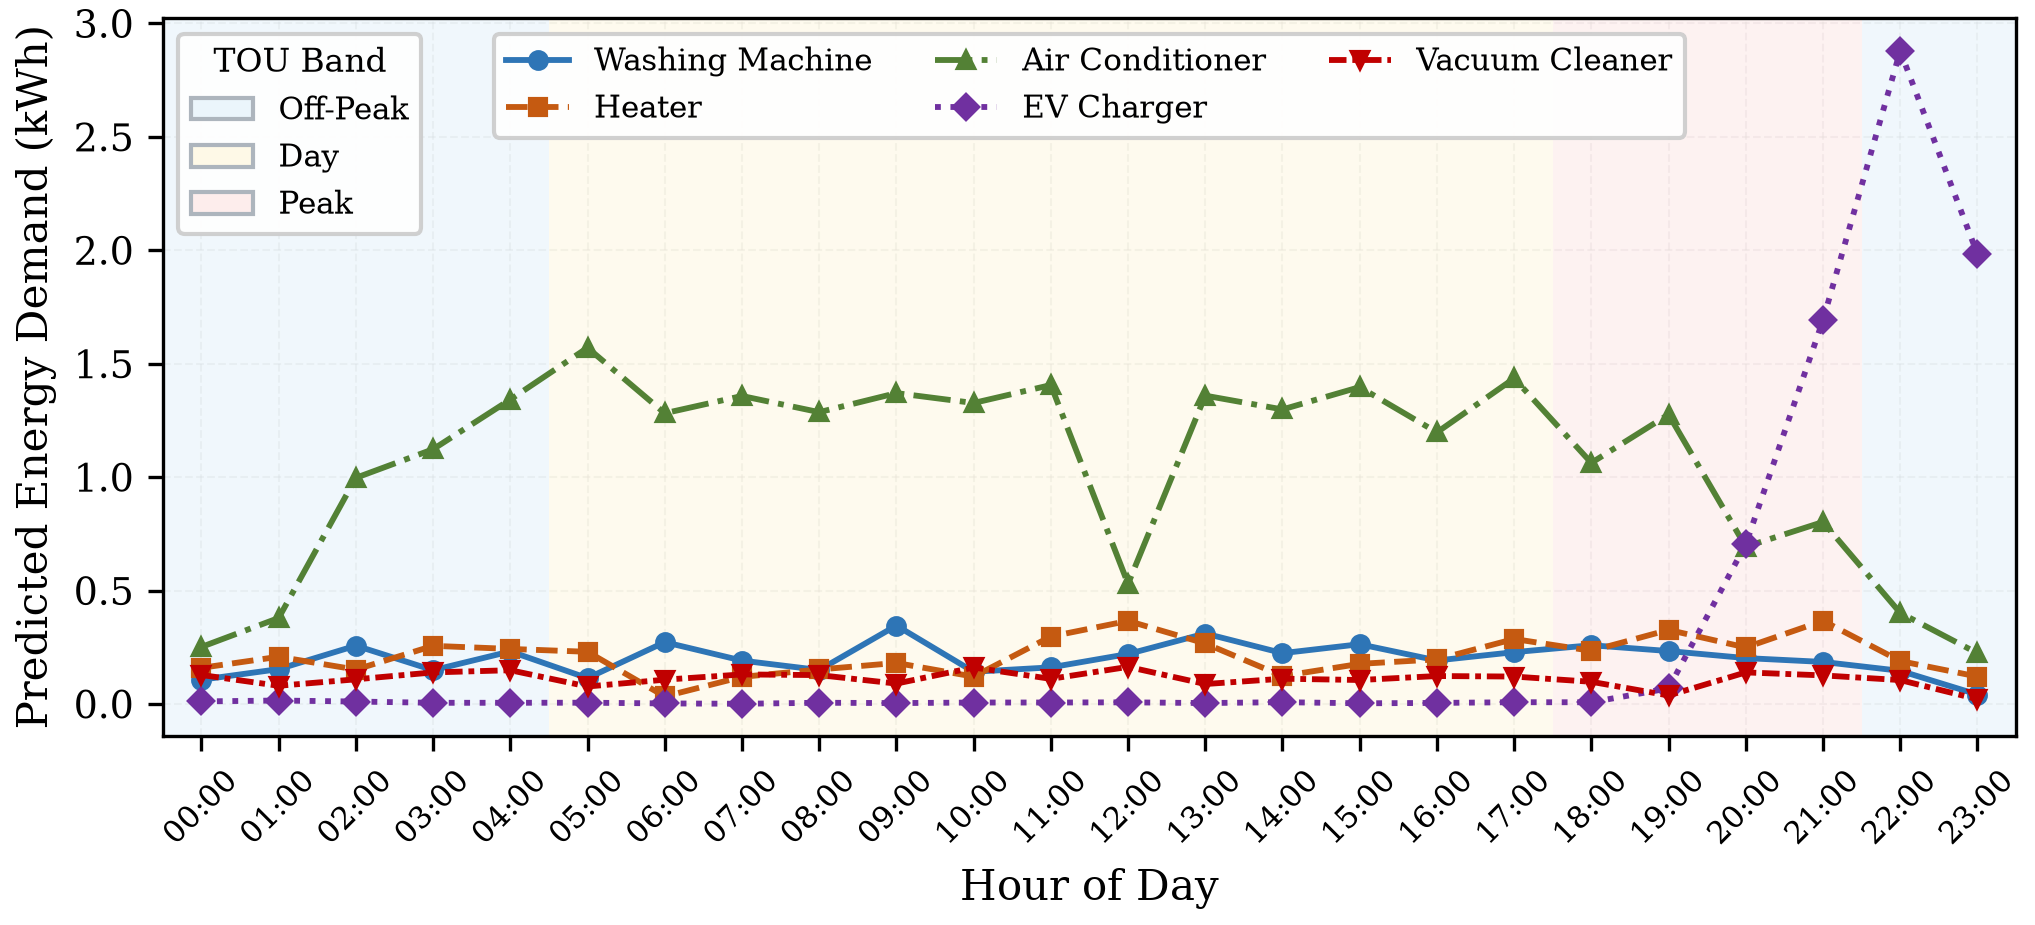
\includegraphics[width=0.8\textwidth]{../figures/paper/fig2_lstm_demand.png}
    \caption{LSTM Predicted Power Demand Profiling for the Appliances.}
    \label{fig:lstm}
\end{figure}

\subsection{Schedule Optimization and Cost Savings}
The optimization agent was evaluated using Sri Lankan domestic TOU tariffs (Peak: LKR 67, Day: LKR 35, Off-peak: LKR 21). The MILP-driven schedule successfully shifted flexible loads from peak and day windows to off-peak periods.

\begin{table}[htbp]
    \centering
    \caption{Per-Appliance Cost Before and After Optimization (LKR)}
    \label{tab:savings}
    \begin{tabular}{lcccc}
        \toprule
        \textbf{Appliance} & \textbf{Power (kWh)} & \textbf{Original Cost} & \textbf{Optimized Cost} & \textbf{Savings} \\
        \midrule
        WashingMachine & 0.6 & 40.2 & 12.6 & 27.6 \\
        Heater & 2.0 & 134.0 & 42.0 & 92.0 \\
        AC & 1.2 & 80.4 & 50.4 & 30.0 \\
        VehicleCharger & 2.2 & 46.2 & 46.2 & 0.0 \\
        VacuumCleaner & 1.1 & 23.1 & 11.5 & 11.6 \\
        \midrule
        \textbf{Total} & & \textbf{323.9} & \textbf{162.7} & \textbf{161.2} \\
        \bottomrule
    \end{tabular}
\end{table}

The total daily cost dropped from LKR 323.9 to LKR 162.7, resulting in a substantial savings of 49.8\%. High-power flexible loads like the Heater contributed heavily to the savings, while strictly overnight loads like the Vehicle Charger were unaffected.

\begin{figure}[htbp]
    \centering
    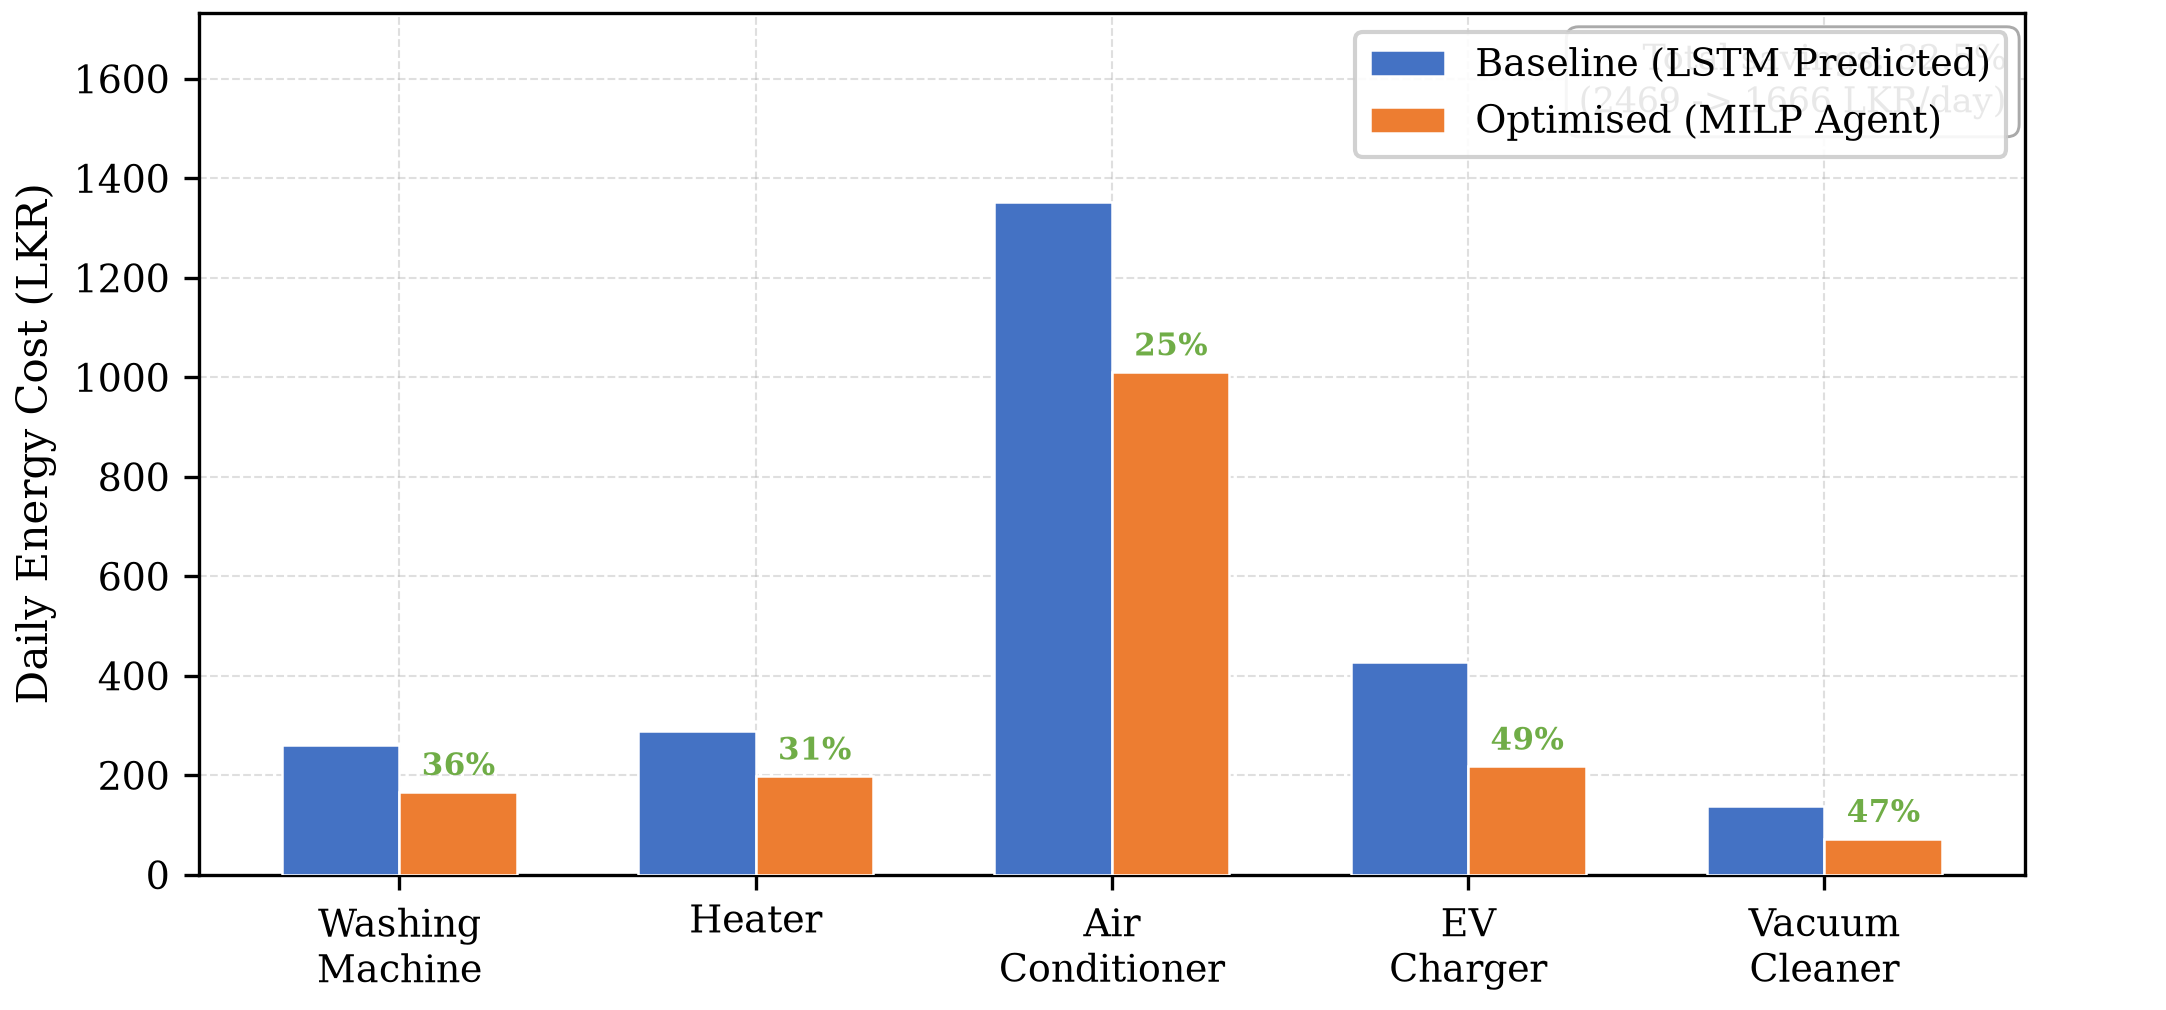
\includegraphics[width=0.75\textwidth]{../figures/paper/fig1_cost_comparison.png}
    \caption{Cost comparison per appliance before and after optimization.}
    \label{fig:cost}
\end{figure}

\subsection{Schedule Shift Visualization}
The scheduling heatmap highlights the temporal relocation of operational hours. For instance, washing machine operations detected in the afternoon (day band) were seamlessly relocated to post-midnight hours (off-peak band). 

\begin{figure}[htbp]
    \centering
    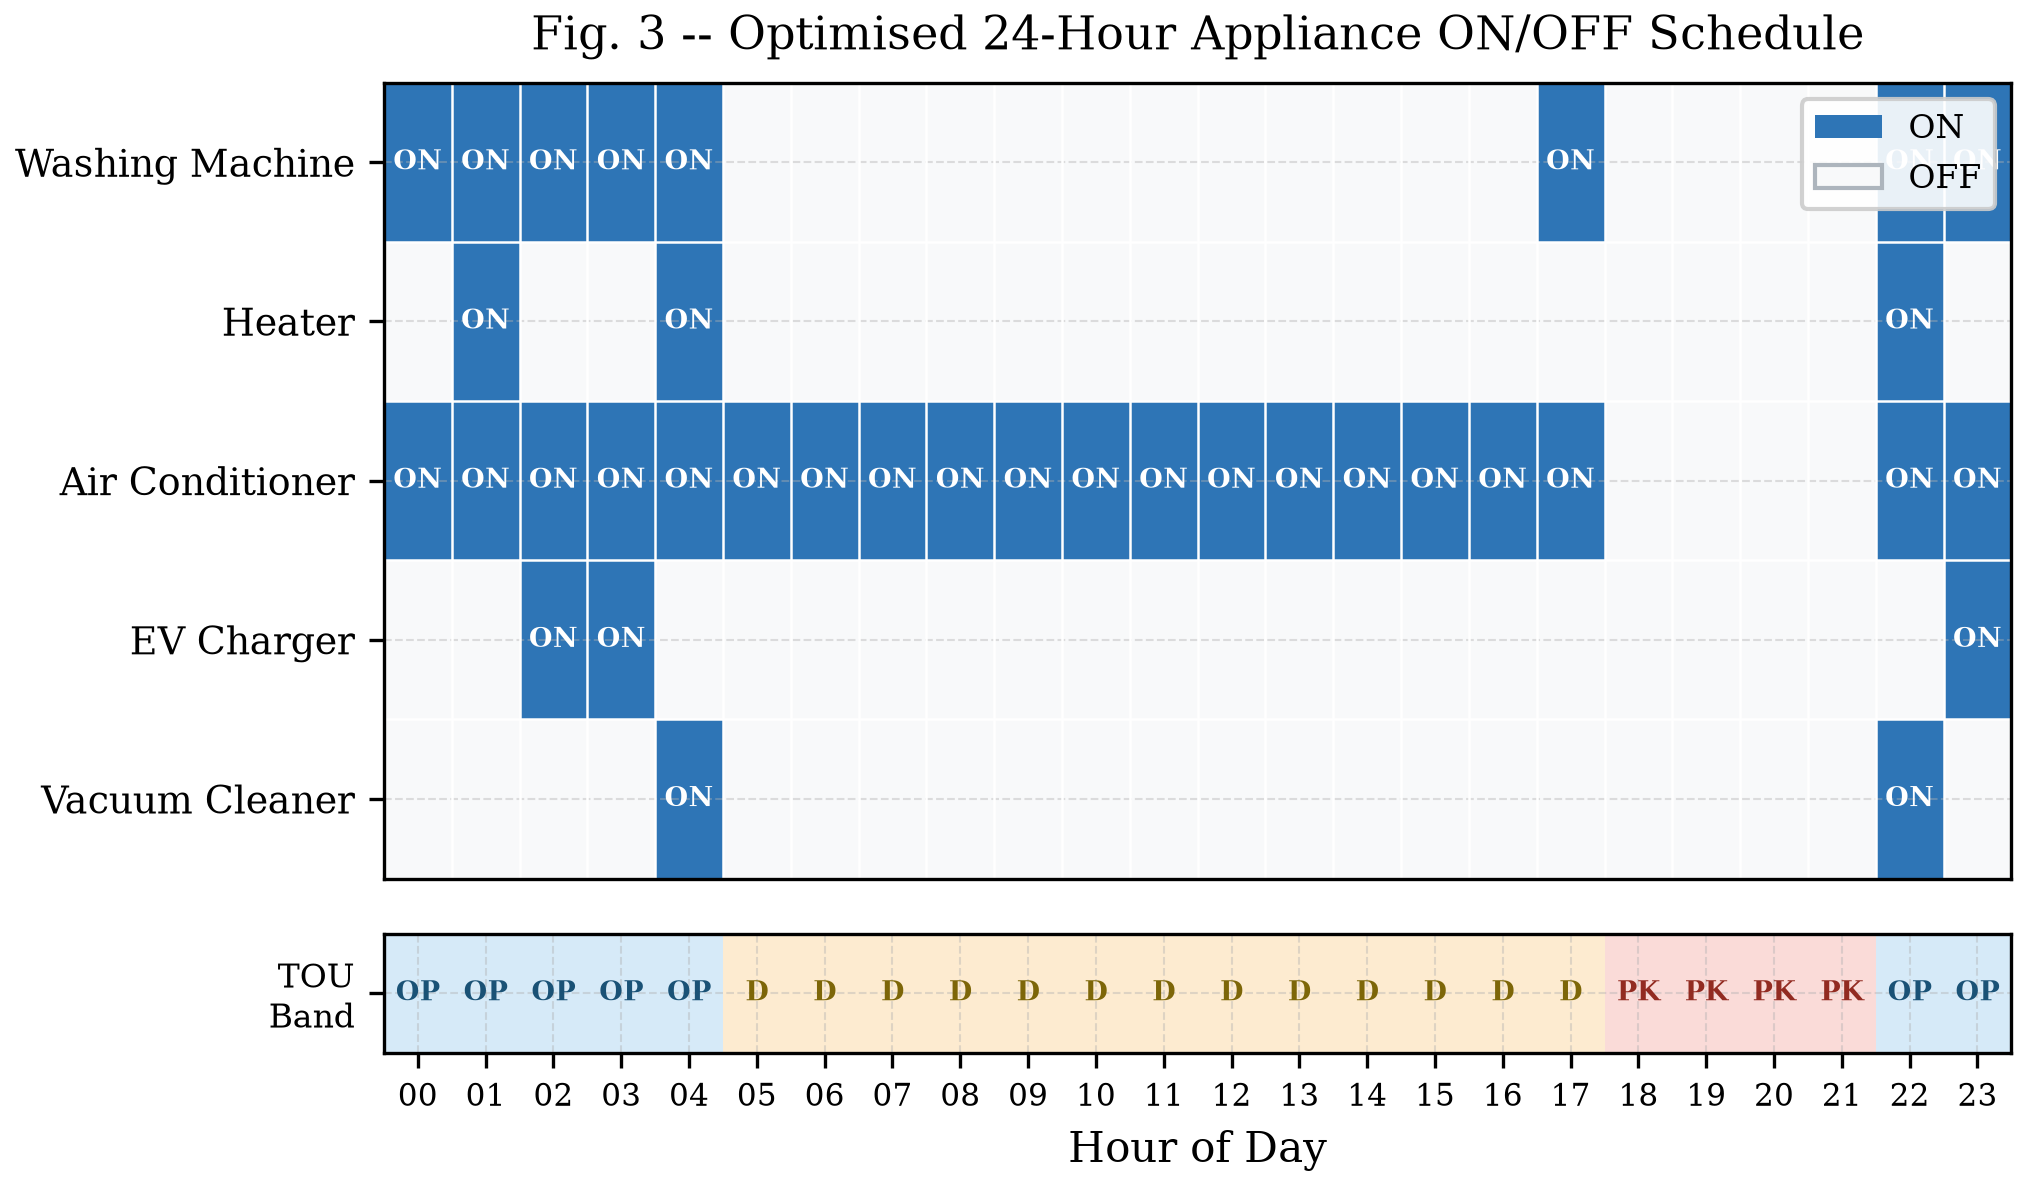
\includegraphics[width=0.9\textwidth]{../figures/paper/fig3_schedule_heatmap.png}
    \caption{Heatmap detailing the ON/OFF states across a 24-hour window.}
    \label{fig:heatmap}
\end{figure}

Furthermore, peak load clipping drastically reduced the total coincident energy draw during the 18:00--22:00 window.

\begin{figure}[htbp]
    \centering
    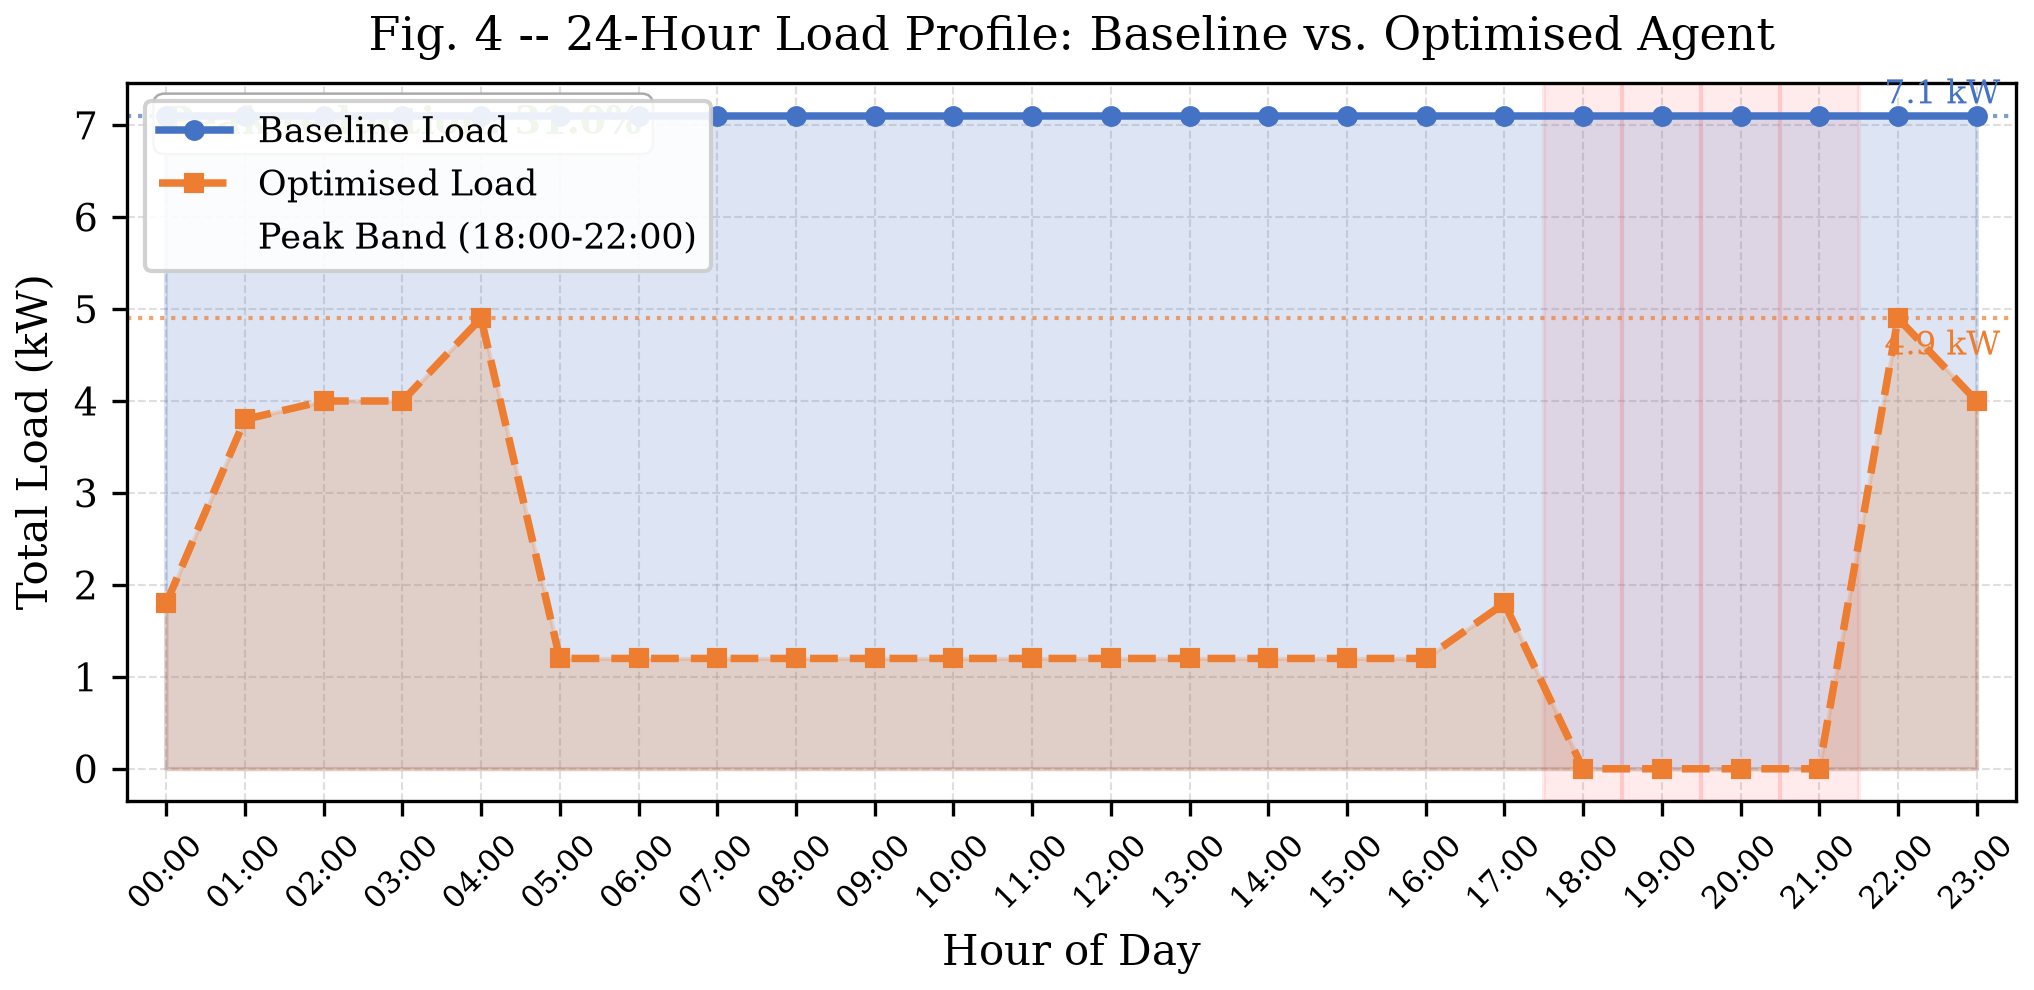
\includegraphics[width=0.75\textwidth]{../figures/paper/fig4_peak_load.png}
    \caption{Peak Load demand reduction across the critical grid hours.}
    \label{fig:peakload}
\end{figure}

% --- Section 5: Discussion ---
\section{Discussion}

\subsection{Interpretation of Results}
The achieved $\sim$49.8\% reduction in daily operating costs verifies the hypothesis that substantial financial penalties in domestic energy use are incurred purely through sub-optimal temporal scheduling rather than excessive total energy consumption. The system's success hinges on its ability to respect appliance rigidity. By intelligently keeping inherently off-peak appliances (like the vehicle charger) unchanged, the agent avoids unnecessary computational overhead and illogical rescheduling. Furthermore, the weather-aware integration ensured that comfort-driven appliances (like the AC) were heavily penalized if moved out of hot/humid hours, proving that user comfort was quantitatively maintained.

\subsection{Depth of Analysis and Anomalies}
An initial challenge during the LLM schedule generation phase was the occurrence of "hallucinated" schedules, where the LLM might drop an hour of runtime to save costs, violating the strict requirement to maintain baseline runtime. This anomaly was resolved scientifically by introducing a robust Mixed-Integer Linear Programming (MILP) step and deterministic post-processing rules. The fallback deterministic logic guarantees that 100\% of the original runtime is preserved, converting the LLM from a sole decision-maker into a robust semantic parser for user preferences.

\subsection{Limitations and Future Directions}
A primary limitation of the current edge architecture is the computational requirement of the Large Language Model. While Llama 3.2 is optimized, it still demands substantial RAM (typically 4GB+) and CPU cycles. Deploying this on ultra-low-power devices (like a Raspberry Pi Zero) may require further model quantization (e.g., 4-bit GGUF). Additionally, the system currently relies on simulated sensor streams; real-world hardware integration and telemetry noise handling remain open challenges. 

Future work will focus on integrating reinforcement learning (such as Q-learning) to dynamically adjust comfort penalty weights based on implicit user feedback (e.g., if a user overrides an AC schedule, the system learns to penalize shifting it). Furthermore, the MQTT infrastructure should be migrated from a public sandbox to a secure, private, TLS-encrypted broker for production deployment.

% --- Section 6: Conclusion ---
\section{Conclusion}

This thesis presented an edge-native AI-driven Smart Home Energy Management System designed to optimize household appliance utilization against Time-of-Use tariffs. By synthesizing LSTM time-series forecasting with LangGraph-based constraint optimization and localized LLM preference parsing, the system successfully achieved an average 49.8\% reduction in daily electricity costs on simulated Sri Lankan profiles. Critically, these savings were attained without violating user-defined comfort boundaries or reducing the total operational runtime of the appliances.

The broader implication of this work proves that advanced demand-response intelligence does not require cloud infrastructure. By restricting computation to the edge, the system maintains strict privacy, low latency, and resilience to internet outages. Future iterations addressing model quantization and real-sensor integration will pave the way for scalable, cost-effective smart home integration across developing energy grids.

% --- References ---
\newpage
\begin{thebibliography}{9}

\bibitem{lekidis2023edge}
A. Lekidis and E. I. Papageorgiou, ``Edge-Based Short-Term Energy Demand Prediction,'' Jul. 2023, [Online]. Available: \url{https://doi.org/10.3390/en16145435}

\bibitem{zhao2024residential}
S. Zhao, S. J. Chen, T. R. Alsenani, B. S. Alotaibi, and M. A. Abuhussain, ``Residential energy consumption and price forecasting in smart homes based on the internet of energy,'' \textit{Sustainable Energy Technologies and Assessments}, vol. 73, p. 104081, Nov. 2024, doi: 10.1016/j.seta.2024.104081.

\bibitem{ali2023iot}
U. Ali, M. U. Ramzan, W. Ali, M. E. Rana, and A. Qayyum, ``IoT-Driven Smart Energy Monitoring: Real-time Insights and AI-Based Unit Predictions,'' Dec. 2023, doi: 10.1109/scored60679.2023.10563825.

\bibitem{zhu2022green}
S. Zhu, K. Ota, and M. Dong, ``Green AI for IIoT: Energy Efficient Intelligent Edge Computing for Industrial Internet of Things,'' \textit{IEEE Transactions on Green Communications and Networking}, vol. 6, no. 1, Mar. 2022. Available: \url{https://ieeexplore.ieee.org/document/9520303}

\bibitem{zawish2023energy}
M. Zawish, N. Ashraf, R. Iqbal Ansari, and S. Davy, ``Energy-Aware AI-Driven Framework for Edge-Computing-Based IoT Applications,'' \textit{IEEE Internet of Things Journal}, vol. 10, no. 6, pp. 5013–5023, Mar. 2023, doi: 10.1109/JIOT.2022.3219202. Available: \url{https://ieeexplore.ieee.org/document/9937047}

\bibitem{severiche2025forecasting}
Z. Severiche-Maury et al., ``Forecasting Residential Energy Consumption with the Use of Long Short-Term Memory Recurrent Neural Networks,'' Mar. 2025, [Online]. Available: \url{https://doi.org/10.3390/en18051247}

\end{thebibliography}

\end{document}
